% The fate of a hypothetical second moon of Earth.
% AASTeX 6.3.1. Build instructions: paper/README.md.
% Numbers quoted here are printed by src/paper_numbers.py and src/analyze_pilot.py.

\documentclass[twocolumn]{aastex631}

\usepackage{xcolor}
\newcommand{\pending}[1]{\textcolor{red}{[#1]}}
\graphicspath{{../figures/}{figures/}}

\shorttitle{A hypothetical second moon of Earth}
\shortauthors{\pending{Author}}

\begin{document}

\title{The Fate of a Hypothetical Second Moon of Earth:\\
N-body Simulations and a Machine-Learning Surrogate}

\author{\pending{Author Name}}
\affiliation{\pending{Program, University, City, Country}}

\begin{abstract}
What would happen if Earth had a second natural satellite? We integrate the Sun, Earth, Moon and
a hypothetical second moon from real initial conditions (JPL Horizons, DE440) and study 12,000
randomly drawn second moons spanning $10^{-3}$ to 1 lunar masses and 0.1 to 3 lunar distances,
on prograde and retrograde orbits, for up to 100 years. The setup reproduces the lunar
ephemeris to within 10.3~km over one year. In the full sample, 38.0\% of second moons survive
100 years, 32.0\% are ejected, 27.4\% collide with Earth and 1.4\% collide with the Moon; in
1.2\% of systems the Moon itself is lost. A controlled pilot study shows that displacing the
second moon by 1~m changes 12\% of outcomes, setting an empirical limit on predictability.
We train machine-learning classifiers to predict the outcome from the initial parameters alone
\pending{and reach an accuracy of X\% against a majority-class baseline of 38.0\%, at a speedup
of Y over direct integration}. The dataset and code are publicly available.
\end{abstract}

\keywords{Natural satellites (Solar system) --- Orbital dynamics --- N-body simulations ---
Astronomy data analysis \pending{add Unified Astronomy Thesaurus identifiers}}

\section{Introduction} \label{sec:intro}

Earth has a single large satellite, but this need not always have been the case. Simulations of
the Moon-forming giant impact can leave additional bound debris \citep{Canup2001}, and
\citet{Jutzi2011} proposed that the lunar farside highlands formed when a companion moon of a few
percent of the lunar mass collided with the Moon. Whether a second moon could persist is a
question of orbital stability in a system perturbed by both the Moon and the Sun.

For satellites of planets, the Sun's tidal field limits stable orbits to a fraction of the
planet's Hill radius, with retrograde orbits remaining stable to larger distances than prograde
ones \citep{Domingos2006, Shen2008}. Near the Moon, mutual perturbations and close encounters add
further instabilities. Mapping these outcomes requires many direct N-body integrations, each of
which can take minutes when close encounters force small time steps.

Machine-learning surrogates offer a faster alternative. \citet{Tamayo2020} showed that a
classifier trained on short integrations predicts the long-term stability of compact planetary
systems orders of magnitude faster than direct integration. Here we apply a similar approach to a
hypothetical second moon of Earth. We (i) validate an N-body setup against the real lunar
ephemeris, (ii) quantify the sensitivity of outcomes to numerical tolerance, initial conditions
and start date in a pilot study, (iii) generate a reproducible dataset of 12,000 integrations, and
(iv) train surrogate models that predict the outcome from the initial parameters.

\section{Methods} \label{sec:methods}

\subsection{Simulation setup and validation}

We use REBOUND \citep{Rein2012} with the adaptive, high-order IAS15 integrator \citep{Rein2015}
at its default tolerance ($\epsilon = 10^{-9}$). Initial state vectors and gravitational
parameters for the Sun, Earth and Moon are taken from JPL Horizons \citep{Giorgini1996} at
2026-01-01 00:00 TDB in the barycentric ecliptic frame, consistent with the DE440 ephemeris
\citep{Park2021}. Bodies are point masses with physical radii used for collision detection, which
is performed along each integration step so that encounters between outputs are not missed.

To validate the setup, we integrate the real three-body system for one year and compare the
Moon's geocentric position with the Horizons ephemeris every 6~hours.

\subsection{Second-moon parameters}

Each second moon is specified by its mass and geocentric orbital elements, converted to a state
vector at the common epoch. Mass $m$ and semi-major axis $a$ are drawn log-uniformly from
$10^{-3}$--$1\,M_{\rm Moon}$ and 0.1--3 lunar distances (38,440--1,153,200~km, or 0.026--0.78
of Earth's Hill radius of $1.48\times10^{6}$~km at the epoch). Eccentricity is uniform on
0--0.8, and the longitude of the ascending node, argument of periapsis and true anomaly are
uniform on 0--360$^\circ$. Inclination relative to the ecliptic is uniform on 0--180$^\circ$, so
retrograde orbits are included and near-planar orbits are well represented (see
Section~\ref{sec:pilot}). The second moon has the Moon's bulk density. Orbits whose periapsis lies
inside Earth's Roche limit for this density,
\begin{equation}
d_{\rm R} = 2.44\,R_{\rm Moon}\left(\frac{M_\oplus}{M_{\rm Moon}}\right)^{1/3}
\approx 18{,}365~{\rm km},
\end{equation}
are redrawn. Each moon uses an independent random generator seeded by the dataset seed and its
index, so the dataset is reproducible regardless of execution order.

\subsection{Outcomes}

Each system is integrated for up to 100 years with outputs every 24~hours and stopped at the
first terminal event. Outcomes are labeled \texttt{hit\_earth} or \texttt{hit\_moon} for
collisions of the second moon, \texttt{ejected} when the second moon is more than
$4.5\times10^{6}$~km ($\approx 3$ Hill radii) from Earth with positive geocentric orbital energy,
\texttt{moon\_lost} when the Moon rather than the second moon is ejected or collides with Earth,
and \texttt{survived} otherwise. Survivors are right-censored: their lifetime is at least 100
years. No run exceeded the computing limit of 600~s or failed.

\subsection{Pilot study} \label{sec:pilot}

Before generating the full dataset, we simulated 100 moons (drawn with isotropic inclinations,
i.e.\ uniform in $\cos i$) under controlled variations: (B) a tighter tolerance,
$\epsilon = 10^{-11}$; (C) the second moon displaced by 1~m; and (D) two other start dates,
2026-05-01 and 2026-09-01, for the first 30 moons. Decision rules were fixed before the results
were examined: keep the default tolerance unless B disagrees with the reference run on more than
three moons beyond the disagreement of C; adopt multiple start dates if D disagrees clearly more
than C; and choose the longest time limit of 10, 30 or 100 years that fits the computing budget.
Confidence intervals for proportions are Wilson score intervals \citep{Wilson1927}.

\subsection{Surrogate models}

\pending{Phase 4: features (orbital elements and/or geocentric state vectors), train/validation/
test split, handling of the two rare classes, Random Forest baseline \citep{Breiman2001},
gradient-boosted trees and a neural network, hyperparameter selection.}

\section{Results} \label{sec:results}

\subsection{Validation}

Over one year, the simulated Moon remains within 10.3~km of the Horizons ephemeris (mean 5.6~km,
about 0.003\% of the Earth--Moon distance; Figure~\ref{fig:validation}), and its mean orbital
period differs by 0.6~s. Omitting the Sun increases the maximum error to 55,535~km. The
relative energy error stays at the $10^{-15}$ level.

\begin{figure}
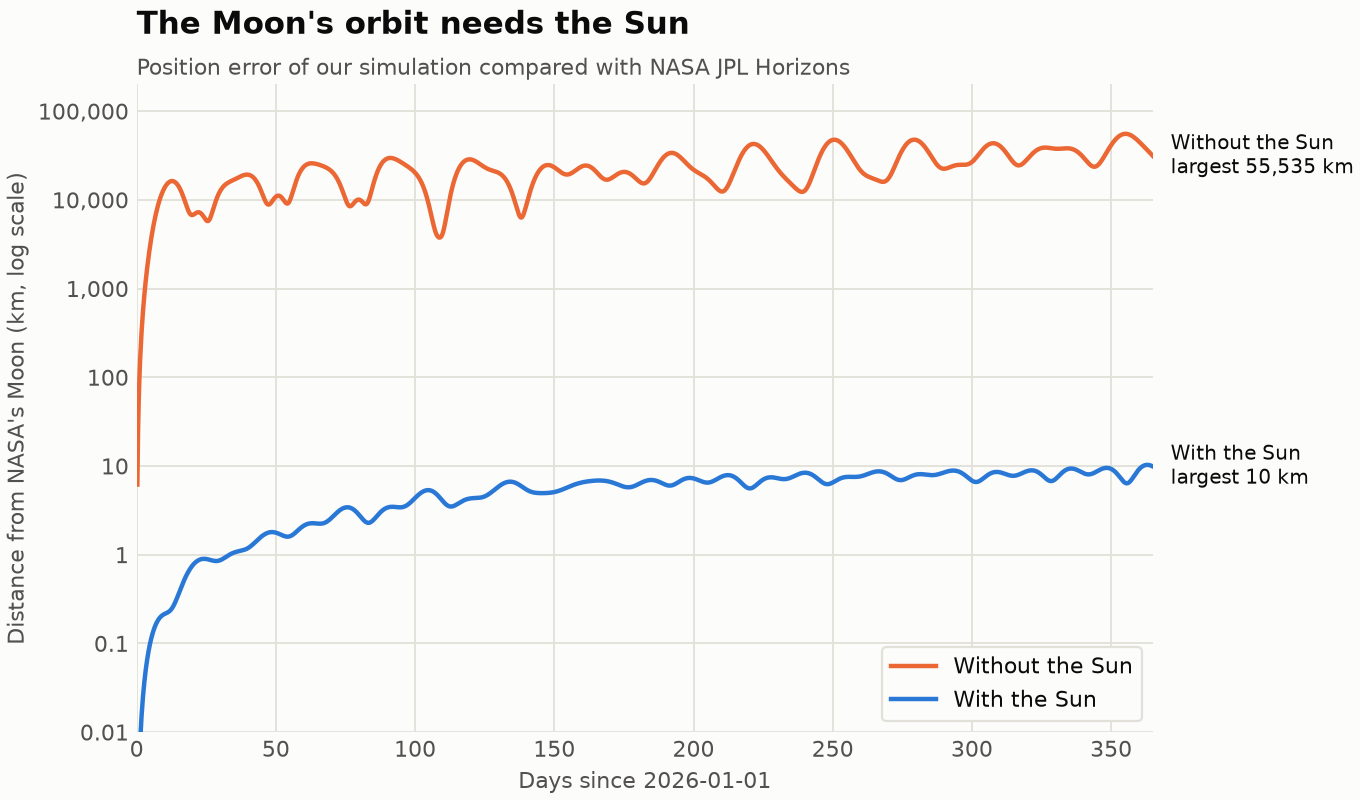
\includegraphics[width=\columnwidth]{real_moon_error.png}
\caption{Distance between the simulated and JPL Horizons positions of the Moon over one year,
with (blue) and without (orange) the Sun. \label{fig:validation}}
\end{figure}

\subsection{Pilot study}

In the reference pilot run, 42 of 100 second moons collided with Earth, 38 were ejected, 18
survived 100 years, one collided with the Moon and in one system the Moon was lost. The surviving
fraction declines steadily with time: 45\% at 10 years, 28\% at 30 years and 18\% at 100 years
(Figure~\ref{fig:survival}).

Displacing the second moon by 1~m changed the outcome of 12 of 100 systems at 100 years
(agreement 88\%, 95\% interval 80--93\%) and 9 at 10 years. Tightening the integrator tolerance
changed 6, fewer than the 1~m displacement, so the default tolerance was kept: the remaining
differences reflect chaotic sensitivity to initial conditions rather than numerical error. The
two alternative start dates agreed with the reference on 27 and 26 of 30 moons, compared with 28
of 30 under the 1~m displacement, showing no clear dependence on the start date. A 100-year
limit fit the computing budget.

Only 7 of the 100 pilot moons had inclinations below 40$^\circ$, consistent with the 11.7\%
expected for isotropic orientations. To cover near-planar orbits better, the full dataset samples
inclination uniformly in degrees. This decision was made after the pilot, and it over-represents
near-planar orbits relative to random orientations.

\begin{figure}
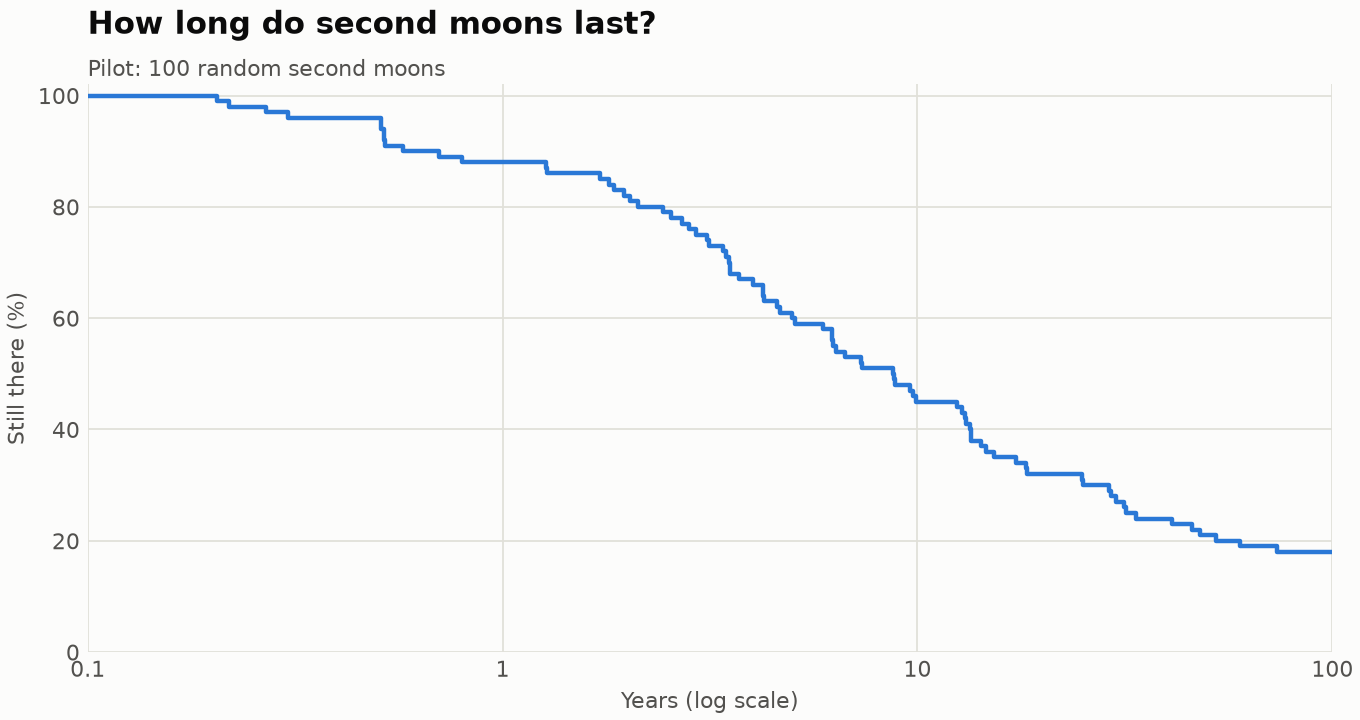
\includegraphics[width=\columnwidth]{pilot_survival.png}
\caption{Fraction of the 100 pilot second moons that have neither collided nor been ejected, as a
function of time. \label{fig:survival}}
\end{figure}

\subsection{Dataset}

The full dataset contains 12,000 systems drawn with an independent seed. It required 20.8
CPU-hours (median 1.5~s and maximum 104~s per system). Table~\ref{tab:outcomes} lists the
outcomes. Automated checks confirm that every input is regenerated exactly from the seed, that
labels are consistent with the raw outcomes, and that re-integrating 20 random systems reproduces
their outcomes and survival times exactly.

\begin{table}
\caption{Outcomes in the full dataset (95\% Wilson intervals). \label{tab:outcomes}}
\begin{tabular}{lrr}
\hline
Outcome & Systems & Share \\
\hline
Survived 100 yr & 4,554 & 38.0\% (37.1--38.8) \\
Ejected & 3,841 & 32.0\% (31.2--32.8) \\
Collided with Earth & 3,288 & 27.4\% (26.6--28.2) \\
Collided with the Moon & 171 & 1.4\% (1.2--1.7) \\
Moon lost & 146 & 1.2\% (1.0--1.4) \\
\hline
Total & 12,000 & \\
\hline
\end{tabular}
\end{table}

The survival fraction (38.0\%) exceeds that of the pilot (18\%, 95\% interval 12--27\%).
\pending{Phase 3: test whether the change in inclination sampling explains the difference.}

\subsection{Stability maps}

\pending{Phase 3: outcome as a function of semi-major axis, inclination, eccentricity and mass;
prograde versus retrograde survival; comparison with the expected limit near half the Hill
radius (about 1.9 lunar distances).}

\subsection{Surrogate performance}

\pending{Phases 4--5: accuracy and per-class metrics on the held-out test set, confusion matrix,
comparison with the majority-class baseline (38.0\%) and with the 88\% agreement rate of the
chaos test, speedup over direct integration, and analysis of misclassified systems.}

\section{Discussion} \label{sec:discussion}

The chaos test sets a practical bound on predictability: if a 1~m change in initial position
alters one outcome in eight, no model of the initial parameters can be expected to predict every
outcome. This bound is indicative rather than strict, since an optimal classifier that predicts
the most probable outcome can exceed the agreement between two noisy realizations.

Outcome shares depend on the sampling design. They describe this dataset rather than the
probability that an arbitrary second moon survives, and the difference between the pilot and the
full dataset illustrates this sensitivity.

The model has several limitations. Bodies interact through Newtonian point-mass gravity only:
tides, Earth's oblateness, general relativity and the other planets are omitted. These effects
are small over the 100-year integrations, as the validation error shows, but they would matter
over longer timescales and for orbits close to Earth. ``Survived'' denotes survival for 100 years,
not long-term stability; in the pilot, the surviving fraction was still declining at that limit.
Finally, a single start date is used, supported by a 30-system test.

\section{Conclusions} \label{sec:conclusions}

\pending{To be completed after Phases 3--5.}

\section*{Data availability}

Code, configuration files and the dataset manifest (including the SHA-256 checksum of the dataset)
are available at \pending{GitHub URL}. The dataset is archived at \pending{Zenodo DOI} and can be
regenerated from the code.

\begin{acknowledgments}
This work made use of the JPL Horizons on-line solar system data service.
\end{acknowledgments}

\software{REBOUND \citep{Rein2012}, astroquery \citep{Ginsburg2019}, Astropy \citep{Astropy2022},
NumPy \citep{Harris2020}, Matplotlib \citep{Hunter2007}}

\bibliography{references}{}
\bibliographystyle{aasjournal}

\end{document}
